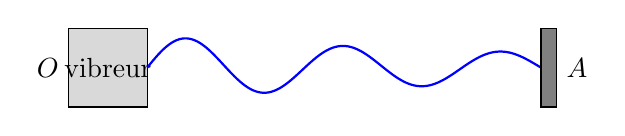
\begin{tikzpicture}[scale=1]
    \draw[fill=gray!30] (-1,-0.5) rectangle (0,0.5);
    \node at (-0.5,0) {vibreur};
    \node[left] at (-1,0) {$O$};
    \draw[thick, blue, domain=0:5, samples=150, smooth]
        plot (\x, {0.4*sin(2*180/2*\x)*exp(-0.15*\x)});
    \draw[fill=gray] (5,-0.5) rectangle (5.2,0.5);
    \node[right] at (5.2,0) {$A$};
\end{tikzpicture}
